\documentclass[12pt]{article}
\usepackage{graphicx}
\usepackage[margin=1in]{geometry}
\usepackage{natbib}
\bibliographystyle{plain}

% Default fixed font does not support bold face
\DeclareFixedFont{\ttb}{T1}{txtt}{bx}{n}{12} % for bold
\DeclareFixedFont{\ttm}{T1}{txtt}{m}{n}{12}  % for normal

% Custom colors
\usepackage{color}
\definecolor{deepblue}{rgb}{0,0,0.5}
\definecolor{deepred}{rgb}{0.6,0,0}
\definecolor{deepgreen}{rgb}{0,0.5,0}
\definecolor{green}{rgb}{0,0.8,0}

% Python style for highlighting
\usepackage{listings}
\newcommand\pythonstyle{\lstset{
language=Python,
basicstyle=\ttm,
otherkeywords={self},             % Add keywords here
keywordstyle=\ttb\color{deepblue},
emph={MyClass,__init__},          % Custom highlighting
emphstyle=\ttb\color{deepred},    % Custom highlighting style
stringstyle=\color{deepgreen},
commentstyle=\color{green},
frame=tb,                         % Any extra options here
showstringspaces=false            % 
}}

% Python environment
\lstnewenvironment{python}[1][]
{
\pythonstyle
\lstset{#1}
}
{}

% Python for external files
\newcommand\pythonexternal[2][]{{
\pythonstyle
\lstinputlisting[#1]{#2}}}

% Python for inline
\newcommand\pythoninline[1]{{\pythonstyle\lstinline!#1!}}


\title{Report 1: Single file diffusion with binding and unbinding \\ PHYC 6261}
\date{March 18, 2016}
\author{Taylor Dunn \\ B00688623}

\begin{document}

\maketitle

\section{Model and Method}

Our model is single file diffusion (SFD) of hard-core particles that cannot pass each other.
Under these conditions, SFD typically exhibits subdiffusive behaviour characterized by mean-squared displacement $<\Delta x^2> \sim t^{1/2}$ \cite{harris1965diffusion}, in contrast with simple-diffusion (SD) scaling of $<\Delta x^2> \sim t$.

% Something about MT acetylation
It has been suggested that the luminal $\rm \alpha TAT1$ protein (radius of 3.5 nm \cite{montagnac2013agr}) may undergo SFD inside microtubules (inner radius of 7 mm \cite{shida2010major}).
%This protein plays an important role in alpha tubulin acetylation.
An important consideration of this diffusive behaviour is the protein binding to sites inside the microtubule, by which it catalyzes the acetylation reaction.

To study the effects of transiently bound particles blocking diffusion, we use stochastic simulations of $N$ particles in a ring geometry (or equivalently, a tube of finite length $L$ with periodic boundary conditions).
The ring is discretized into a lattice with $L$ points, and particle positions and states are updated at each time step as follows:

\begin{enumerate}
    \item If enough time has passed, bind/unbind a random free/bound particle
    \item Choose a random particle.
    \item If the particle is free, choose a random step direction ($\pm 1$).
    \item If the new position is unoccupied, move the particle. 
    \item Update time by $\Delta t = 1/N$.
\end{enumerate}

The choice of time step here ensures that at integer steps of time, each particle has, on average, attempted to move once.
To implement the dynamics of binding and unbinding events, we introduce binding and unbinding rates $K_{\rm on}$ and $K_{\rm off}$, respectively, and employ the Gillespie algorithm to determine the next event and when it occurs:

\begin{enumerate}
    \item Compute the combined rate of the entire system:
    % free particles times binding rate plus bound particles times unbinding rate
    \begin{equation}
        \Gamma = N_f K_{\rm on} + N_b K_{\rm off}
    \end{equation}
    \item Determine the time of the next event:
    \begin{equation}
        t_{\rm next} = t - (1/\Gamma) \log{[\rm RAN(0,1)]}
    \end{equation}
    \item Determine the probability of a binding event versus unbinding:
    \begin{equation}
        P_b = N_f K_{\rm on} / \Gamma
    \end{equation}
\end{enumerate}

For easier comparision of simulation parameters, we also introduce the occupancy number $p = N / L$ and the ratio $R = K_{\rm on} / K_{\rm off}$.


There are multiple approaches to initializing the system (e.g. all particles free, all particles equally spaced, all lattice sites having $p$ probability of being occupied), but for the results presented here, the following process was used:
\begin{enumerate}
    \item Compute the number of bound and free particles as $N_b = N R / (1+R)$ and $N_f = N - N_b$.
    \item For each bound particle, place it at an unoccupied site on the ring.
    \item For each free particle, place it at an unoccupied site on the ring.
\end{enumerate}

At this initial stage of the project, we are exploring the following parameter space:

\begin{table}[!h]
\begin{center}
\begin{tabular}{c c c c}
    Parameter & Primary & Secondary & Fixed \\
    $K_{\rm on}$ & $10^{-3}, 10^{-2}, 10^{-1}, 10^0, 10^1, 10^2, 10^3$ & $10^{-2}, 10^{-1}, 10^0$ & $10^{-1}$ \\
    $R$ & 0.1, 0.2, 0.5, 1, 2, 5, 10 & 0.1, 1, 10 & 1 \\
    $p$ & 0.1, 0.2, 0.3, 0.4, 0.5, 0.6, 0.7, 0.8, 0.9 & 0.1, 0.5, 0.9 & 0.5 \\
\end{tabular}
\caption{The parameter space to be tested. Each member of the class was assigned a primary and secondary variable range to explore.}
\end{center}
\end{table}

The primary goal of this project is to examine how these parameters affect the behaviour of particles undergoing SFD.
An important preliminary step, however, is to determine appropriate system size $L$ to avoid finite-size effects, equilibration time $t_{\rm eq}$ to avoid initial transients, and maximum simulation time $t_{\rm max}$ to ensure that the system has equilibrated to its final behaviour.

\newpage

\section{Results}

For a system with periodic boundary conditions, care must be taken to avoid finite-size effects.
Ring sizes ranging from $L = 10$ to $L = 400$ were simulated up to $t_{\rm max} = 10^4$ at the fixed parameter values in Table 1, and the mean squared displacement with statistical error bars are plotted in Figure 1.
To achieve good statistics, and sample the same overall number of particles, averages were taken over varying numbers of runs $M$ such that $N = pLM = 10^4$.

\begin{figure}[h]
    \centering
    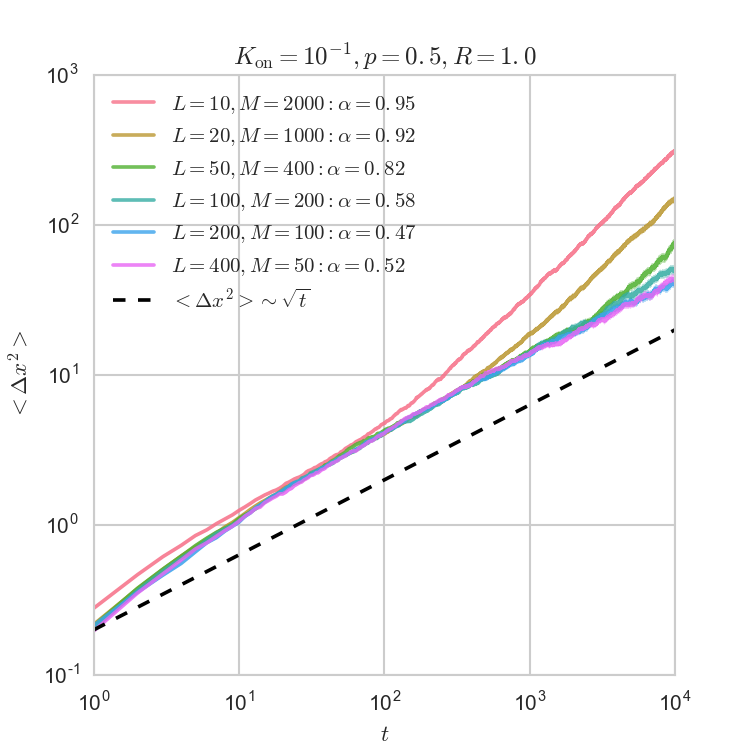
\includegraphics[width=0.8\linewidth]{../plots/L_dependence.png}
    \caption{Mean squared displacement ($\pm$ SEM) vs. time with varying system size $L$. Each set of data was fit to $<\Delta x^2> = A t^{\alpha}$, and best fit estimates for $\alpha$ are listed in the legend. Also plotted is a reference line corresponding to the familiar SFD result $<\Delta x^2> \sim \sqrt{t}$.}
\end{figure}

At intermediate times (between $t = 10$ and $10^3$), most of the data appears to scale as expected for SFD ($\sim \sqrt{t}$), but all of the data besides $L = 200$ and 400 looks to reach a diverging point where the particles exhibit superdiffusive ($\alpha > 0.5$) behaviour.
This diverging point is earlier for smaller system sizes.
From this result, we can conclude that a system size of $L = 200$ is an appropriate choice for this time scale, and for our fixed parameters.

\newpage

Figure 1 raises another question: what is causing the super-diffusive behaviour at early times?
One explanation is that the initial condition (randomly placed particles, bound/free ratio $R$) is not in equilibrium, so the system requires an equilibration time to reach its steady state before measurements should be taken.
Figure 2 shows averages from $M = 100$ simulations for equilibration times ranging from $t_{\rm eq} = 0$ to $10^4$.

\begin{figure}[h!]
    \centering
    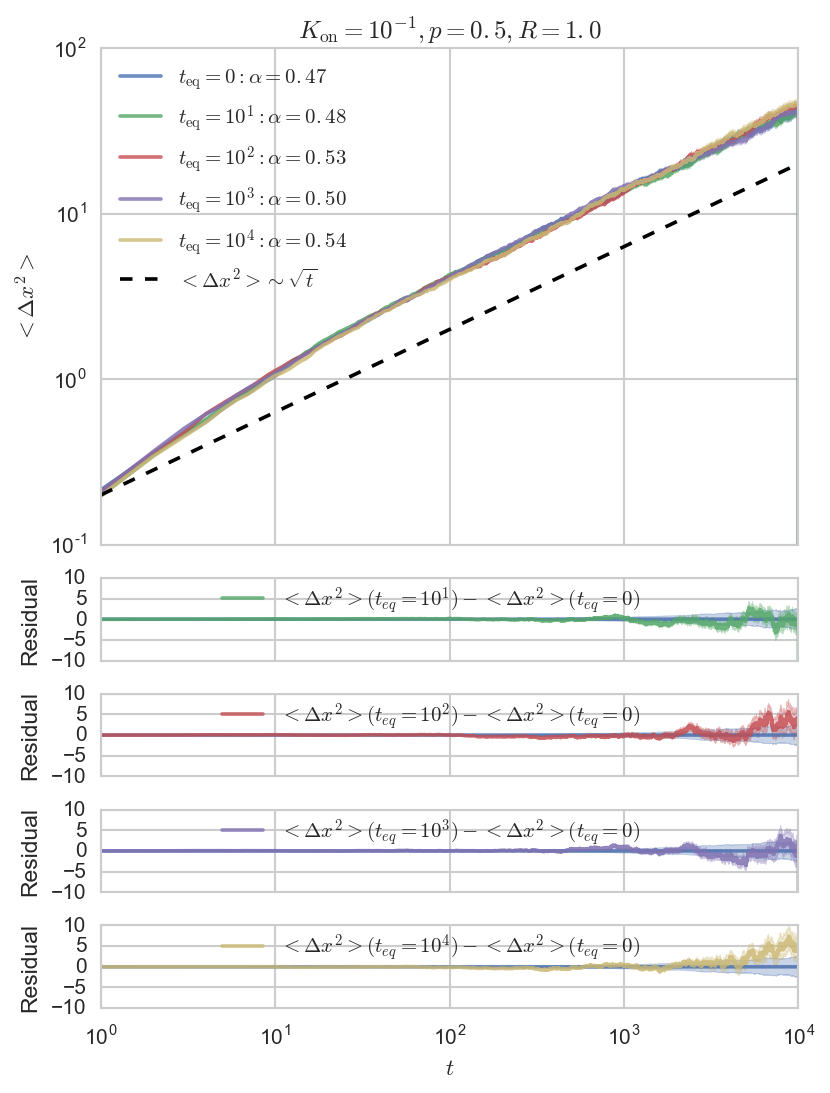
\includegraphics[width=0.8\linewidth]{../plots/teq_dependence_resid.png}
    \caption{Mean squared displacement ($\pm$ SEM) vs. time with varying equilibration time $t_{\rm eq}$. Each set of data was fit to $<\Delta x^2> A t^{\alpha}$, and best fit estimates for $\alpha$ are listed in the legend. Plotted below are the residuals of the displacement compared to $t_{\rm eq} = 0$.}
\end{figure}

Despite some minor fluctuations at late times, the data lie on top of each other.
This suggests that the initial condition has little to no effect on the measurement of $<\Delta x^2>$, and consequently the best way to avoid the transient regime is to ignore it and only fit to data after a certain time 
For these parameters, it would appear that time is around $t > 10^2$.

As with any experiment, especially a collaborative one with independent simulation code, reproducibility is essential.
Plotted in Figure 3 are sets of data from simulations ran by different group members at fixed parameter values.
While there is disagreement at late times, especially compared to JP's data, this may just be due to statistical fluctuations at such large length scales.
More cross-comparisons should be done at different parameter values to further ensure reproducibility.

\begin{figure}[h!]
    \centering
    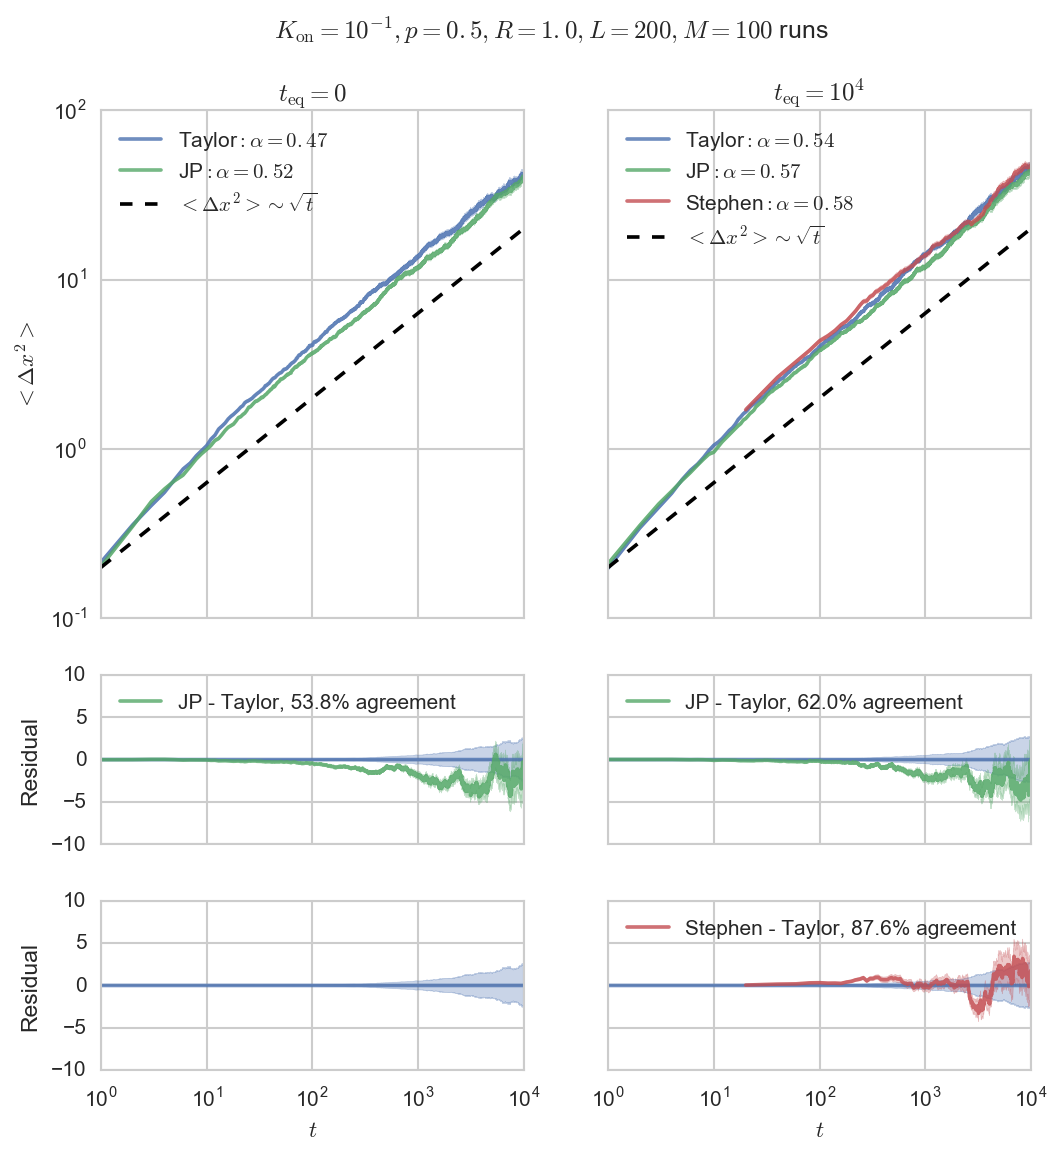
\includegraphics[width=0.8\linewidth]{../plots/group.png}
    \caption{Mean squared displacement ($\pm$ SEM) vs. time from simulations ran by different group members. Each set of data was fit to $<\Delta x^2> = A t^{\alpha}$, and best fit estimates for $\alpha$ are listed in the legend. Plotted below are the residuals of the displacement compared to Taylor's data, along with percent agreement within error bars.}
\end{figure}

\newpage

With preliminary analysis complete, we now move on to exploring the parameter space of $K_{\rm on}$ primary and $p$ secondary.
A system size $L = 200$ was used, and $M = 100$ simulations were averaged to produce the data presented in Figure 4.
\begin{figure}[h!]
    \centering
    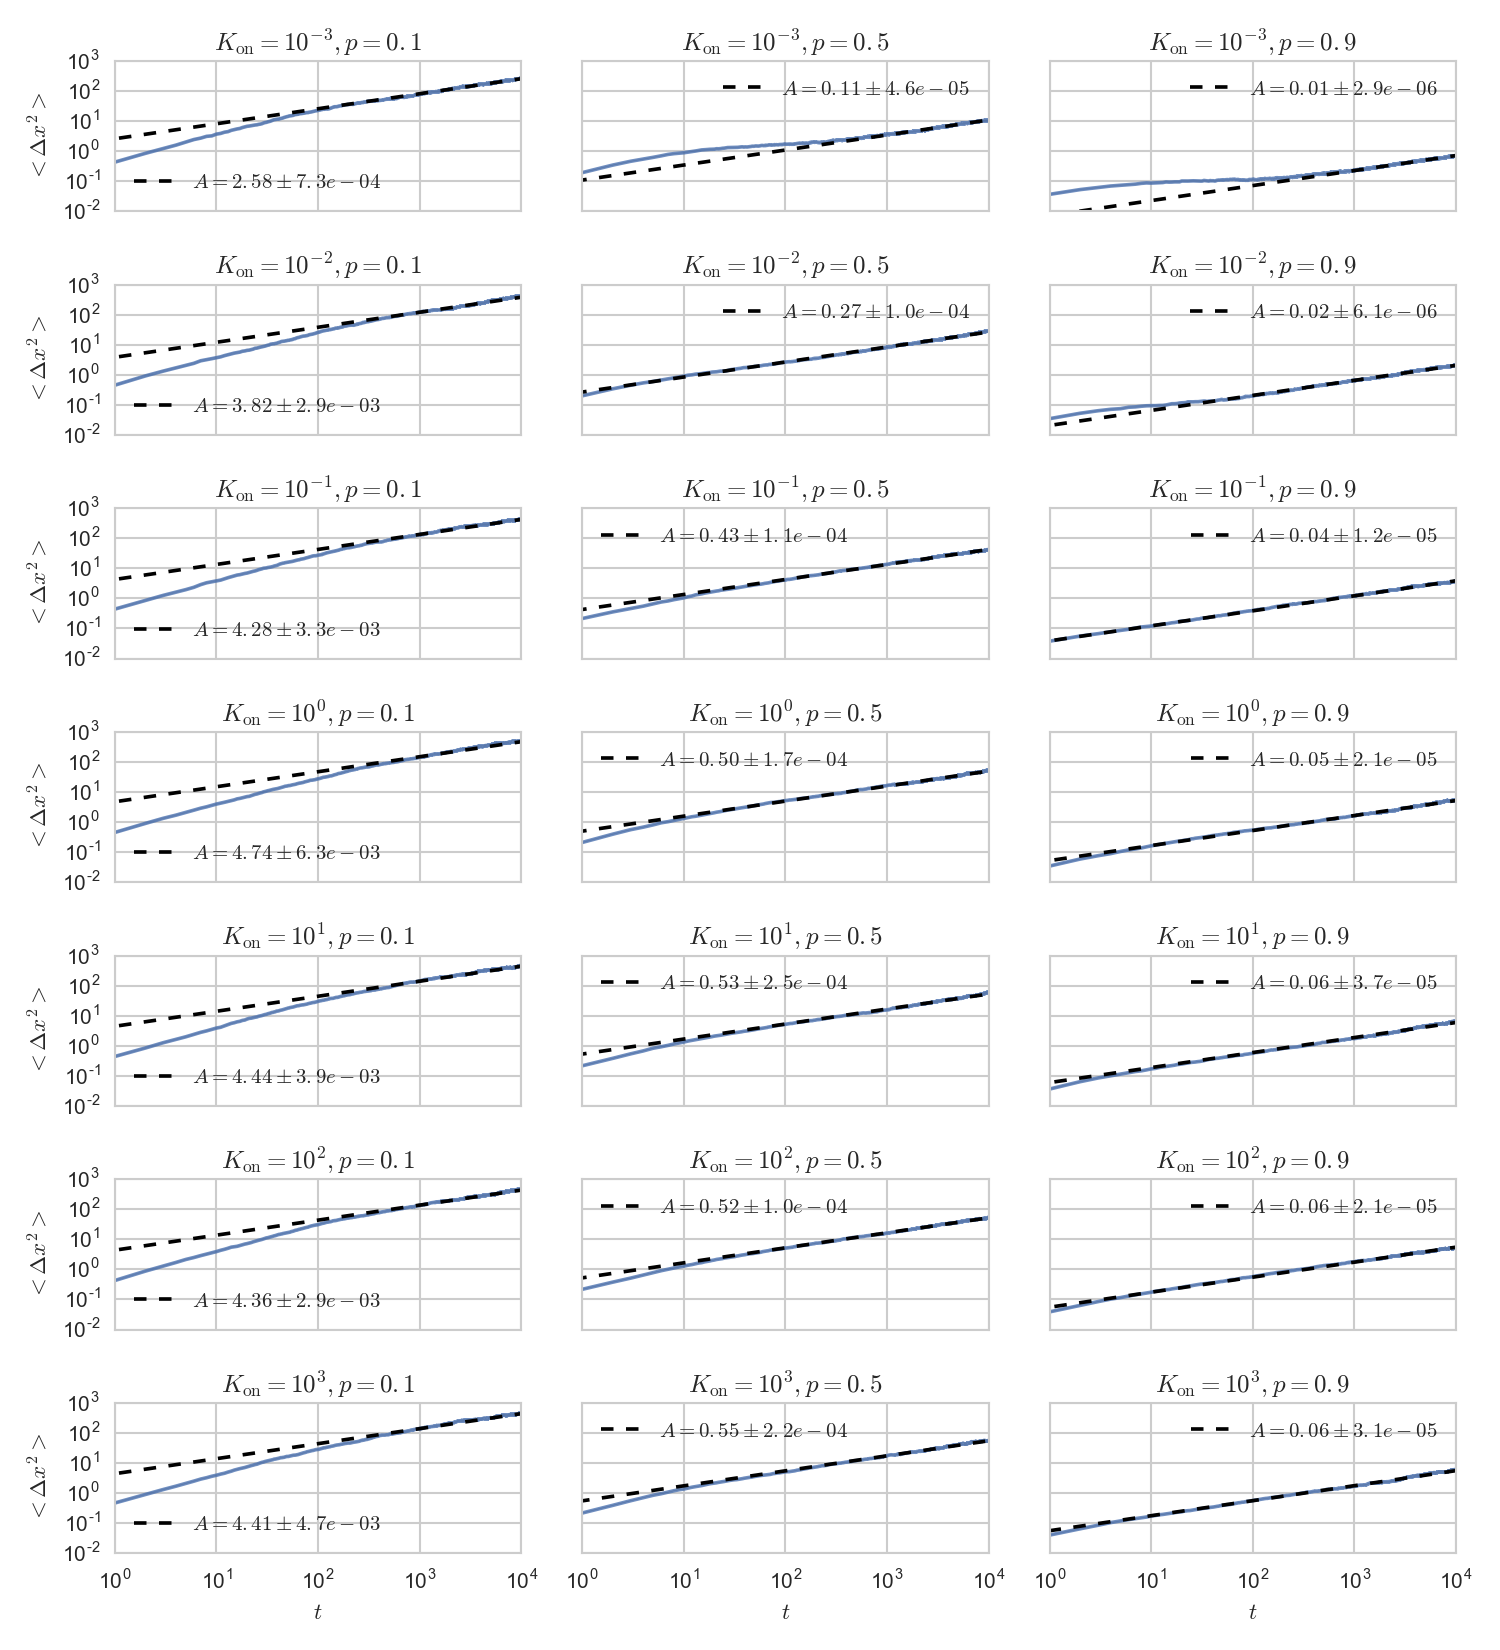
\includegraphics[width=\linewidth]{../plots/param_space.png}
    \caption{Mean squared displacement ($\pm$ SEM) vs. time for varying $K_{\rm on}$ and $p$ values. Each set of data was fit to $<\Delta x^2> = A \sqrt{t}$ for $t > 10^2$, and best fit estimates for the prefactor $A$ are listed.}
\end{figure}

\newpage

An immediate observation from the above figure is that the initial super-diffusive behaviour lasts longer for $p = 0.1$, up to $t = 10^3$ at high values of $K_{\rm on}$.
A possible explanation is that at lower densities, particles have more space to diffuse before running into other particles and "settling" to their steady-state behaviour.
This may lead us to using a larger $t_{\rm max}$ for low $p$ values in the future, but this should not affect the estimated fit parameters here significantly.
Curiously, mean squared displacement for $K_{\rm on} = 10^{-3}$ and $p = 0.5, 0.9$ (also $K_{\rm on} = 10^{-2}$ and $p = 0.9$ to a lesser degree) seems to exhibit sub-diffusive ($\alpha < 0.5$) behaviour at early times.
This should certainly be investigated further, and for smaller values of $K_{\rm on}$ than the range presented here.

The fit prefactors $A$ are plotted versus $K_{\rm on}$ and $p$ in Figure 5 below.

\begin{figure}[h!]
    \centering
    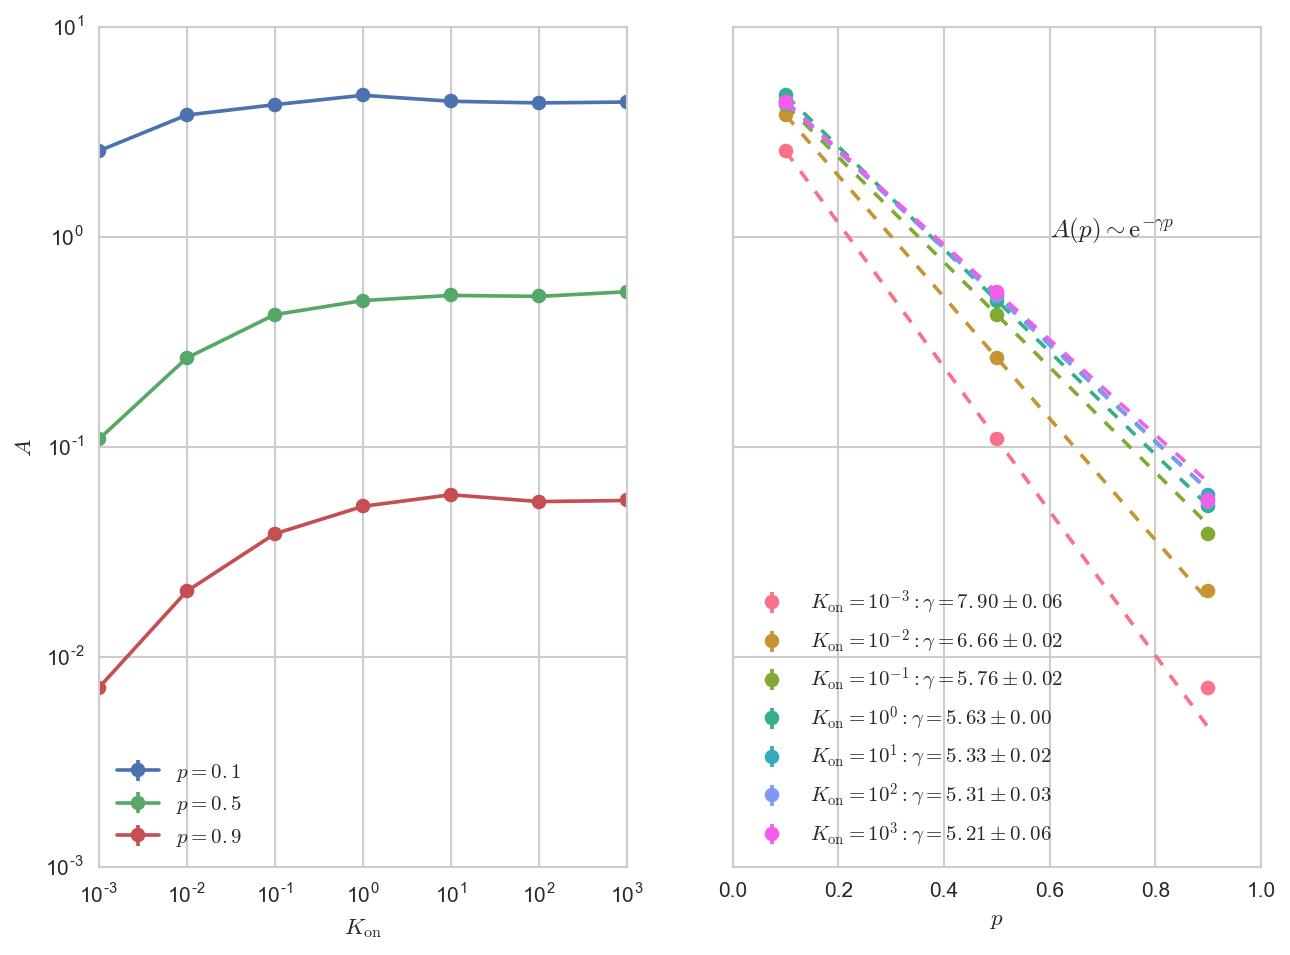
\includegraphics[width=\linewidth]{../plots/param_space_fits.png}
    \caption{Prefactors $A$ ($\pm$ error from the least squares fit) from Figure 4. $A$ vs. $p$ was fit to an exponential decay and the decay rates $\gamma$ are listed in the legend.}
\end{figure}

With increasing $K_{\rm on}$, $A$ asymptotically approaches a constant, the value of which increases with decreasing $p$.
This tells us that beyond $K_{\rm on} = 10$, the binding and unbinding rates are so fast that no difference can be discerned in the diffusive behaviour.
A more appropriate $K_{\rm on}$ range to explore may be from $10^{-5}$ (or so) to $10^1$.
From both plots, it is clear that $A$ decreases with $p$.
This is expected because for high density, particles have less room to diffuse and thus have a smaller "amplitude" of displacement.
Although only 3 values of $p$ were tested here, there is evidence of some scaling behaviour of $A$ with $p$ -- specifically, it looks to be exponentially decaying.
It will be interesting to compare the results of varying $p$ primary and $K_{\rm on}$ secondary by Stephen, and investigate this relationship further.

\section{Simulation code}

\pythonexternal{../code/simulate.py}


\bibliography{report1.bib}
\end{document}
